% ============================================================================================
% PAPER 1, SHORT FORMAT (PRL) -- VERSION 2 (2026-10-19, user): story led by geometry over topology, with the coherent flow as what lets geometry act
% and elongation acting by disrupting that flow. Version 1 (flow-alignment framing) stays in main.tex. Body unchanged except one sentence (lambda in ellipses).
% Scope (user, 2026-10-13): cavities only; the channel appears once, as the flat limit of the wall law.
% Length target: PRL 3750 words incl. captions (~4 figures). Current draft: see `texcount` (TODO).
% Numbers come from reports/theory_report (26 pp, 2026-10-14) and RESEARCH.md. Every
% "TODO" marks a decision or a missing piece; "%%" comments give the figure plan.
% Figures: placeholders reuse the report's vector PDFs; the final figures are composites (see plan).
% Origin of every number: NUMBERS.md (audit 2026-10-15). Update it with any new or changed number.
% ============================================================================================
\documentclass[aps,prl,twocolumn,superscriptaddress,amsmath,amssymb,reprint]{revtex4-2}
\usepackage{graphicx}
\usepackage{xcolor}
\usepackage[hidelinks]{hyperref}
\graphicspath{{figs/}{../../theory_report/figs/}}
\DeclareGraphicsExtensions{.pdf,.png}
\newcommand{\half}{\tfrac12}
\newcommand{\la}{\ell_a}
\newcommand{\kT}{k_BT}
\newcommand{\todo}[1]{\textcolor{red}{[TODO: #1]}}

\begin{document}

\title{Geometry, not topology, places the charge of active nematic cavities}
%% v2 alternatives: "Confined active flow lets geometry, not topology, place topological charge"; "Active flow sorts topological charge by the geometry of the wall";
%% "Why an active nematic cavity holds one charge in its bulk". v1: "Flow alignment sets the topological charge of active nematic cavities"
\author{Benjamin Loewe}
\affiliation{Facultad de F\'isica, Pontificia Universidad Cat\'olica de Chile, Santiago 7820436, Chile}
\author{Tyler N. Shendruk}
\affiliation{School of Physics and Astronomy, The University of Edinburgh, Peter Guthrie Tait Road, Edinburgh EH9 3FD, United Kingdom}
\date{\today}

\begin{abstract}
A cavity whose wall anchoring winds $k$ times must hold topological charge $k$, but topology does not say where. A passive nematic places all $2k$ half-integer
defects at the wall. An active nematic keeps exactly $2k-2$ there and moves a net charge $+1$ into the bulk. Using particle-based simulations and continuum theory,
we show that the geometry of the anchoring selects this split, and that the coherent flow of the confined active nematic is what lets it act. The anchoring has
$2k-2$ homeotropic sites and ties each wall defect's tilt to its position, so only a ring of $2|k-1|$ defects can tilt as a whole. The active vortex imposes such
a common tilt, at the flow-aligned angle in the no-slip shear at the wall, and a ring of $2k$ must eject two defects. The tilt also turns each wall defect's active
jet along the wall. Elongating the cavity breaks the coherent vortex; the wall defects lose their common tilt, their jets turn inward, and the layer leaks until the
bulk holds a fixed charge per unit wall length. Reversing the winding adds up to two $-\half$ to the wall instead, and these layers, without jets, do not leak.
\end{abstract}
\maketitle

% --------------------------------------------------------------------------------------------
%% INTRODUCTION (~4 paragraphs). TODO(Benjamin): framing and literature; below is a placeholder argument.
Confining an active nematic turns its chaotic flows into coherent ones: circulating vortices in disks, laminar or dancing states in channels
\cite{Doostmohammadi2018,Theillard2017,Opathalage2019,Shendruk2017,Hardouin2019}, and active boundary layers at the walls \cite{Hardouin2022}. Anchoring at the walls also fixes the total topological charge, and patterned anchoring lets one impose any winding $k$.
A passive nematic satisfies this constraint at the wall. An active nematic, as we show, does not: in a circular cavity of winding $k$ it keeps
$2k-2$ defects of charge $+\half$ at the wall and sends a net $+1$ into the bulk, for $k=2$--10 and cavity radii from $0.8$ to $\approx2.2$ active lengths ($\approx2.0$ for larger $k$).
Norton \emph{et al.}\ imposed boundary charges $-1$, 0 and $+1$ on continuum active nematics in disks and found the dynamics insensitive to topology: in the
turbulent state the boundary charge is held in a thin topological boundary layer around a neutral interior \cite{Norton2018}. Klein \emph{et al.}\ imposed larger
windings on disks, up to $q=5$ (ten $+\half$ defects), with activity kept below the threshold for spontaneous pair creation; the defects then braid in periodic or chaotic
orbits and, as in earlier simulations of disks and annuli, tend to screen the excess charge near the boundary \cite{Klein2026}. In experiments on confined
microtubule nematics the wall defects are $-\half$, and $+\half$ are ejected into the bulk \cite{Hardouin2022}. Here we impose windings up to $k=10$ (20 $+\half$)
in the regime of continual pair creation, and find that the boundary does not screen the excess charge completely: exactly $+1$ always enters the bulk, and in
non-circular cavities far more. Topology is screened, geometry is not.
%% Novelty check 2026-10-19: Norton2018 (full text: tangential +1 and aster/neutral/saddle; net charge in a boundary layer, neutral interior, no case with bulk net charge),
%% Klein2026 (arXiv v3 full text: winding q up to 10/2, pair creation suppressed, no wall/bulk counts; screening statement cites Norton2018 and an experimental disk paper),
%% Hardouin2022; Semantic Scholar "cited by": Norton2018 57, Hardouin2022 40, Klein2026 0 -- none reports a 2k-2 wall layer with a bulk +1. Closest new work: Fang2026
%% (Leslie angle selected at walls by active flow, no anchoring) -> cited in the tilt paragraph. Also related: Vafa et al. 2023 (cones, imposed charge), Houston 2025
%% (elastic anisotropy in active nematics), Ienaga et al. 2025 (elongated MDCK confinement: vortex -> oscillation with aspect ratio; possible citation for the shape transition).

Here we identify the mechanism, and it is geometric. The winding of the anchoring creates $2k-2$ homeotropic sites on the wall and ties each wall defect's tilt
to its position, so a ring of $2k-2$ defects can tilt as a whole by sliding along the wall, while a ring of $2k$ cannot. Geometry alone does not act, however: in a passive
cavity the $2k$ ring is stable. What activates it is the coherent vortex of the confined active nematic, which imposes a common tilt; the $2k$ ring then ejects two
defects, and a passive cavity under an imposed vortex does the same. The angle of the tilt is the flow-aligned angle in the no-slip shear, $\arccos(1/\lambda)$. In
elongated cavities the vortex breaks, the common tilt is lost, and the untilted wall defects propel themselves into the bulk, even at strong flow alignment; with the
winding reversed the same geometry adds up to two $-\half$ to the wall, and these layers, which have no jets, do not leak.

% --------------------------------------------------------------------------------------------
\paragraph*{Model.} We simulate a two-dimensional active nematic with multi-particle collision dynamics (MPCD, NIAMH-MPCD \cite{Kozhukhov2022}): extensile active
dipoles, activity $\zeta=0.07$ (active length $\la=22.2$ cells, measured as in Ref.~\cite{Kozhukhov2024}), measured Frank constants $K_1\approx42\,\kT$ (splay) and $K_3\approx23\,\kT$ (bend), and flow-alignment
parameter $\lambda=2$ unless stated. No-slip walls impose strong anchoring with director angle $\theta=k\phi$ along the wall (uniform in arclength for non-circular walls).
Cavities are circles of radius $R=0.2$--$2.9\,\la$ with $k=2$--10, and ellipses and Cassini ovals of aspect ratio 1.1--2.5 at three sizes (675 runs). Details in the SM.

% --------------------------------------------------------------------------------------------
%% FIG. 1 (composite, full width): (a) passive vs active density maps (maps_circles a, d-f); (b) anchoring sketch with 2k-2 homeotropic points and the lock (fig_lock);
%% (c) wall count and bulk charge vs R/l_a for k = 2..10 (TODO: new panel from the circle sweep, server seeds); (d) snapshot with tilted wall defects and the vortex (TODO).
\begin{figure*}[t]
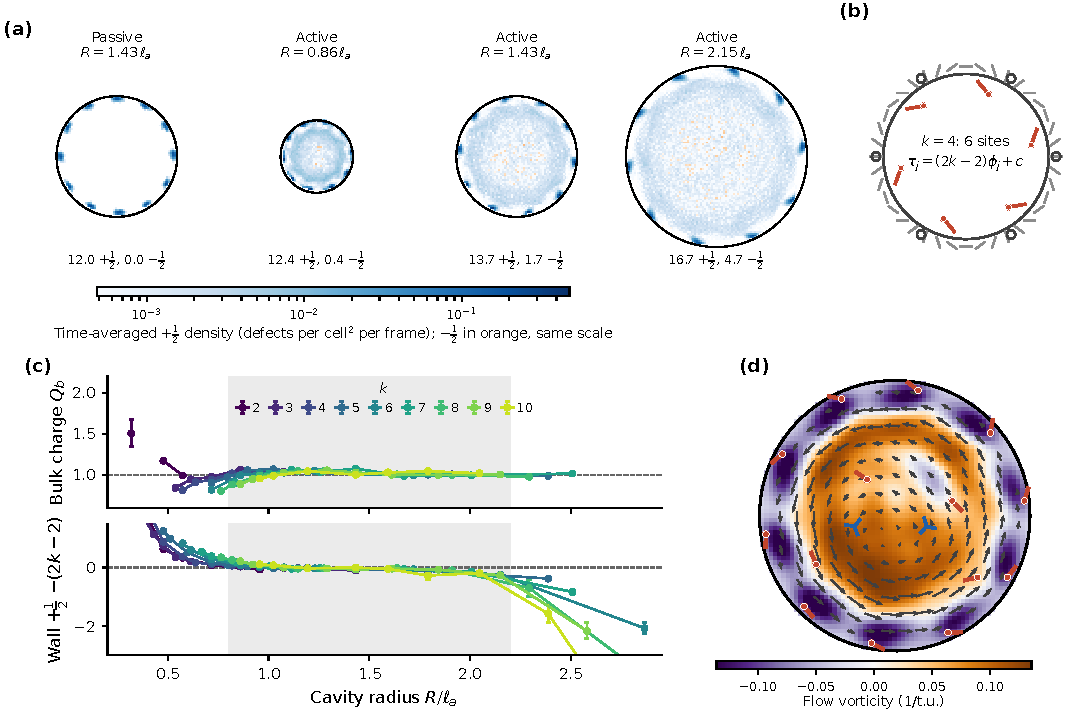
\includegraphics[width=\textwidth]{fig1_observation}
\caption{Overcharging of active circular cavities. (a) Time-averaged defect density ($k=6$, log scale; $+\half$ blue, $-\half$ orange): passive, all $2k=12$ $+\half$ at
the wall; active, $2k-2=10$ wall sites plus dynamic bulk defects. (b) Anchoring with winding $k$ ($k=4$): $2k-2$ homeotropic sites (circles); the lock ties each wall
defect's tilt to its position. (c) Bulk charge (knee of the cumulative charge) and wall $+\half$ count minus $2k-2$ against $R/\la$, $k=2$--10, mean $\pm$ s.e.\ over
10 seeds; shaded: $0.8\le R/\la\le2.2$. (d) Snapshot ($k=6$, $R=1.43\,\la$): flow vorticity and velocity, one vortex, a tilted wall layer.}\label{fig:obs}
\end{figure*}

\paragraph*{Observation.} In passive cavities all $2k$ $+\half$ defects sit in a ring at the wall (Fig.~\ref{fig:obs}). With activity, and for $0.8\lesssim R/\la\lesssim2.2$, the wall
holds exactly $2k-2$ sharply localised defects and the bulk a net charge $+1$, while $\pm\half$ pairs are created and annihilated in the bulk. A single vortex fills
the cavity, and the wall defects are tilted by $61$--$66^\circ$ from the wall normal at low wall density, all in the sense of the vortex. This holds on average over $k=2$--10 and $0.8\le R/\la\le2.2$ (510 runs, 10 seeds each; wall occupancy 0.997, bulk charge $1.01$), with $k$-dependent edges (Fig.~\ref{fig:obs}c).

\paragraph*{Anchoring geometry.} Relative to the local wall normal the anchored director turns by $(k-1)\phi$, so it is homeotropic at $2k-2$ points
$\phi_n=2\pi n/(2k-2)$. A wall $+\half$ at azimuth $\phi_j$ has its tail tilted from the normal by
\begin{equation}
\tau_j=(2k-2)\phi_j+\text{const},\label{eq:lock}
\end{equation}
which the simulations obey with a mean resultant length 0.99. Tilt and position are one degree of freedom: a common tilt of a ring is a rigid shift of its registry.
A ring of $2k-2$ defects can therefore sit untilted on the homeotropic points, and tilt as a whole at no elastic cost. A ring of $N=2k$ evenly spaced defects cannot:
by Eq.~\eqref{eq:lock} consecutive tilts differ by $-2\pi/k$ and wind twice around the ring. With unequal splay and bend constants the commensurate ring is pinned
to the sites (barrier 80--110\,$\kT$ at $k=6$), and the incommensurate one is not.

% --------------------------------------------------------------------------------------------
%% FIG. 2 (mechanism): (a) energy of the ejected structure vs the 2k ring under a common tilt (tilted_structures b); (b) passive cavity + imposed vortex: wall count and
%% tilt coherence vs time (fig_ejection); (c) continuum active Q-tensor with backflow: same state (TODO: snapshot panel from shear_tilt/active_bf).
\begin{figure}[t]
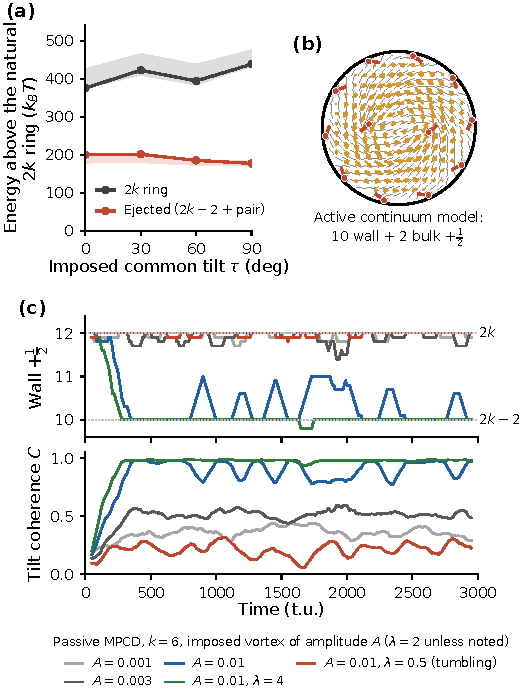
\includegraphics[width=\columnwidth]{fig2_mechanism}
\caption{Flow-induced ejection ($k=6$). (a) Elastic energy above the $2k$ ring with its natural, winding tilts, when every wall defect is forced to a common tilt
$\tau$: the $2k$ ring (grey) and the ejected structure, $2k-2$ ring plus a bulk pair (red); lines: $K_1/K_3=1.82$; bands: elasticities and core sizes.
(b) Active continuum model with backflow, started from the passive ring: one vortex, $2k-2$ wall defects, bulk $+1$. (c) Passive MPCD under an imposed vortex of
amplitude $A$: wall count and tilt coherence. Ejection follows a common tilt and is absent for a tumbling nematic.}\label{fig:eject}
\end{figure}

\paragraph*{Flow-induced ejection.} A coherent flow imposes a common tilt on the wall defects. For the commensurate ring this is free; for the ring of $2k$ it costs
375--475\,$\kT$ of elastic energy at $k=6$ (200--510\,$\kT$ for $k=4$--8), about twice the 180--200\,$\kT$ needed to move two $+\half$ into the bulk. Ejecting two defects leaves the largest ring that
can tilt uniformly and puts $+1$ in the bulk. Three tests show that the flow, not activity as such, is the cause. A \emph{passive} cavity under an imposed vortex
ejects exactly two defects once the flow is strong enough to impose a common tilt (tilt coherence 0.90--0.98), but not for a tumbling nematic, which has no aligned
angle (Fig.~\ref{fig:eject}). A passive continuum Q-tensor model driven by the measured flow reproduces the thresholded ejection without fitting. An active continuum model with
backflow, started from the passive ring, organises itself into the same state: one vortex, $2k-2$ wall defects, bulk $+1$.

% --------------------------------------------------------------------------------------------
%% FIG. 3 (tilt law): (a) flat-wall sketch: zero mode + Leslie angle (TODO: schematic); (b) tilt vs lambda in active MPCD circles with arccos(1/lambda) (fig_tiltlaw a);
%% (c) imposed-flow variants: shear only in / removed from the wall band (shear_tilt c); (d) inset: wall count vs lambda (fig_tiltlaw b).
\begin{figure*}[t]
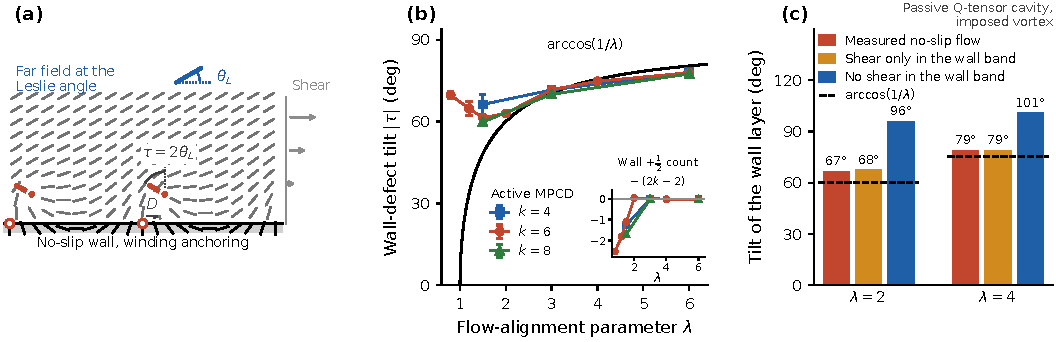
\includegraphics[width=\textwidth]{fig3_tiltlaw}
\caption{Origin of the tilt. (a) Flat no-slip wall with winding anchoring (one-constant solution): sliding the screening $+\half$ by $D$ from a homeotropic site
rotates the far field by $\kappa D$ and the defect by $2\kappa D$; in shear the far field settles at the Leslie angle $\theta_L$, so $\tau=2\theta_L=\arccos(1/\lambda)$.
(b) Wall-defect tilt in active MPCD circles (mean $\pm$ s.e.\ over seeds); inset: wall count minus $2k-2$. (c) Passive Q-tensor cavity under an imposed vortex:
tilt for three flow profiles.}\label{fig:tilt}
\end{figure*}

\paragraph*{The tilt angle.} Elasticity alone would tilt the layer by only $\approx35^\circ$ (a defect-particle model with the computed $K_1\neq K_3$ pinning). The angle comes from flow alignment in the shear next to the no-slip
wall. Consider a flat wall in simple shear with the anchoring winding along it. Translating the screening defect by $D$ rotates the far-field director by $\kappa D$
and the defect by $2\kappa D$ at no energy cost, which is Eq.~\eqref{eq:lock} as a zero mode. Far from the wall the director must sit at the Leslie angle
$\theta_L$ of the shear, $\cos2\theta_L=1/\lambda$. If the layer passes on no torque it slides along its zero mode until the far field is aligned, so
\begin{equation}
\tau=2\theta_L=\arccos(1/\lambda),\label{eq:tilt}
\end{equation}
independent of the shear rate and the elastic constants; only the ratio of strain to vorticity, fixed by the no-slip wall, enters. Active flows alone can select the
Leslie angle at a wall without any anchoring \cite{Fang2026}; here the anchoring is fixed, and the flow acts on the layer through its zero mode. Flat-wall continuum simulations
confirm each step. Removing the shear next to the wall in the cavity model changes the tilt by 29$^\circ$ at $\lambda=2$ and 22$^\circ$ at $\lambda=4$ (above the ejection threshold), while confining all shear to the wall band leaves it
unchanged. In active MPCD circles the tilt follows Eq.~\eqref{eq:tilt} within $3^\circ$ for $\lambda=2$--6: 63.0, 71.7, 74.8, 77.9$^\circ$ against 60.0, 70.5, 75.5,
80.4$^\circ$ at $k=6$, and the same agreement for $k=4$ and 8 at $\lambda=3$ and 6 (Fig.~\ref{fig:tilt}). Below $\lambda\approx2$ the overcharged state itself breaks down, in two ways: small cavities cannot impose a common tilt and keep nearly all $2k$ defects
(at $R_\mathrm{eq}=0.5\,\la$ the full state needs $\lambda=3$), while large ones stay coherent but leak, as the jet route below implies.
Equation~\eqref{eq:tilt} is the flow-dominated limit reached by sparse layers. In crowded layers the tilt falls below it, to $\approx42^\circ$ at a wall-defect spacing of 7 cells
($\lambda=2$), in active and passive layers alike; the fall is ordered by the core depth in units of the alignment length and disappears at large $\lambda$
(15$^\circ$ at $\lambda=2$, $<1^\circ$ at $\lambda=6$, between spacings of 17 and 7 cells) [SM].

% --------------------------------------------------------------------------------------------
%% FIG. 4 (beyond circles): (a) phase diagram: tilt coherence and vacancies vs aspect (phase_shapes c,a); (b) escape mechanism: wall-blocked jet g(d) and the untilting
%% run-up (jetmap c + etsg a, or a sketch); (c) wall law: bulk charge per unit length vs aspect, coloured by q, with the channel point (fig_perlength a or c);
%% SHIELDING (user, 2026-10-14; Japan-poster construction): potential of one bulk +1/2 from the layer alone, circle (3D surface, flat floor) vs aspect-2 ellipse
%%     with the measured depleted layer (wells at vacancies) -> panel (a') or a separate Fig. 4 row; source bulkdyn/fig_shielding_layer (a, c, f).
%% (g) MIRROR CONTROL: done 2026-10-19 (shapes/shape_runs_mirror.csv, mirror_summary.txt).
\begin{figure*}[t]
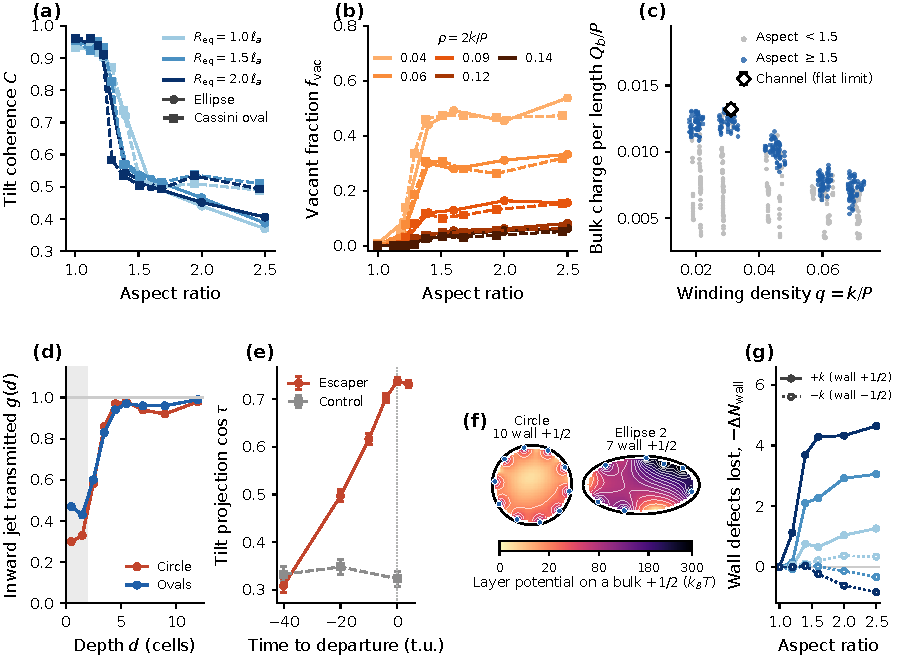
\includegraphics[width=\textwidth]{fig4_shapes}
\caption{Beyond circles. (a) Tilt coherence and (b) vacancies of the wall layer against aspect ratio for ellipses (solid) and Cassini ovals (dashed) at three
sizes. (c) Bulk charge per unit wall length against winding density $q=k/P$; elongated cavities (blue) collapse on a wall law, and the periodic channel (diamond)
is its flat limit. (d) Fraction of a wall $+\half$'s inward jet transmitted near the no-slip wall. (e) Escaping defects untilt over $\approx40$\,t.u.\ before
leaving; residents do not. (f) Potential of a bulk $+\half$ from measured layers (range inside the 0.6 level): $\approx16\,\kT$ in the circle, $\approx180\,\kT$ in the depleted ellipse.
(g) Mirror control: wall defects lost relative to the circle for $+k$ (wall $+\half$, solid) and $-k$ (wall $-\half$, dotted) in the same ellipses (sizes as in (a)).}\label{fig:shapes}
\end{figure*}

\paragraph*{Beyond circles: the layer leaks.} Elongating the cavity breaks the single coherent vortex at aspect ratio 1.25--1.37 for ellipses and ovals alike,
at every size; the active continuum model shows a similar transition (aspect 1.4--1.6). The wall layer then loses defects one at a time. Following single escapes shows why the
tilt matters: each wall $+\half$ is self-propelled along its head, but the tilt turns its jet along the wall, and the no-slip wall transmits only 30--45\%
of the inward component within two cells (the wall-side vortex lobe of the defect is erased). An escaping defect first untilts over $\approx40$\,t.u., its jet
turns inward, and it runs away against an intact elastic barrier. Stronger flow alignment does not prevent this: aspect-2 ellipses keep 2.0--2.8 vacancies at every
$\lambda$ from 2 to 6, because without a coherent vortex there is no common tilt to align. The depleted layer is a unique dynamical steady state, not an elastic one: runs started with 4, 7
or 10 wall defects converge to $7.2\pm0.1$ (aspect 2, $k=6$), although moving a bulk $+\half$ into a gap would lower the elastic energy by 80--100\,$\kT$. Exits slow as the
layer empties (0.068 per wall defect per 20\,t.u.\ for a full layer, 0.028 with five vacancies; elongated cavities, aspect 1.4--2), and this sets where losses and refills balance.

In a circle the evenly spaced layer shields the bulk completely: with same-sign wall images, the potential a bulk $+\half$ feels from the layer is flat
inside the ring apart from a corrugation next to it (a two-dimensional shell theorem: an ideal ring leaves 1.6\,$\kT$ inside $r<0.6R$, measured full layers $\approx17\,\kT$; Fig.~\ref{fig:shapes}(f)).
Elongation alone weakens this only to 14--27\,$\kT$ (without/with the flux of the imposed winding), and fewer but evenly spaced wall defects only to $\approx27\,\kT$ (ranges inside the 0.6 level). The measured layers of aspect-2
ellipses are both depleted and unevenly spaced, and they do not shield at all: the potential tilts across the interior by 180--230\,$\kT$ (median inside the 0.6 level; same bracket), downhill
towards the largest gaps. \todo{trim; decide main text vs SM; the other bulk charges, absent here, partly screen this field}

In the circle the same construction explains the wall exchange. A full, count-locked layer leaves $\approx17\,\kT$ of field inside $r<0.6R$; a single vacancy or an
extra wall defect is an unscreened half-charge whose logarithmic field ($\approx140\,\kT$) spans the cavity, and with a vacancy it points at the hole in every
measured frame (Fig.~\ref{fig:vac}). Accordingly, an entry into the layer triggers an exit 4--5 times sooner than chance (median 22 vs 99\,t.u.), usually of
another defect anywhere on the ring. \todo{CHECK with Benjamin before using: the maps show no potential drop near some layer defects and an asymmetry in the circle; tips of ellipses look unusually well shielded (see RESEARCH.md 2026-10-14 'TO REVIEW')}
\begin{figure}[t]
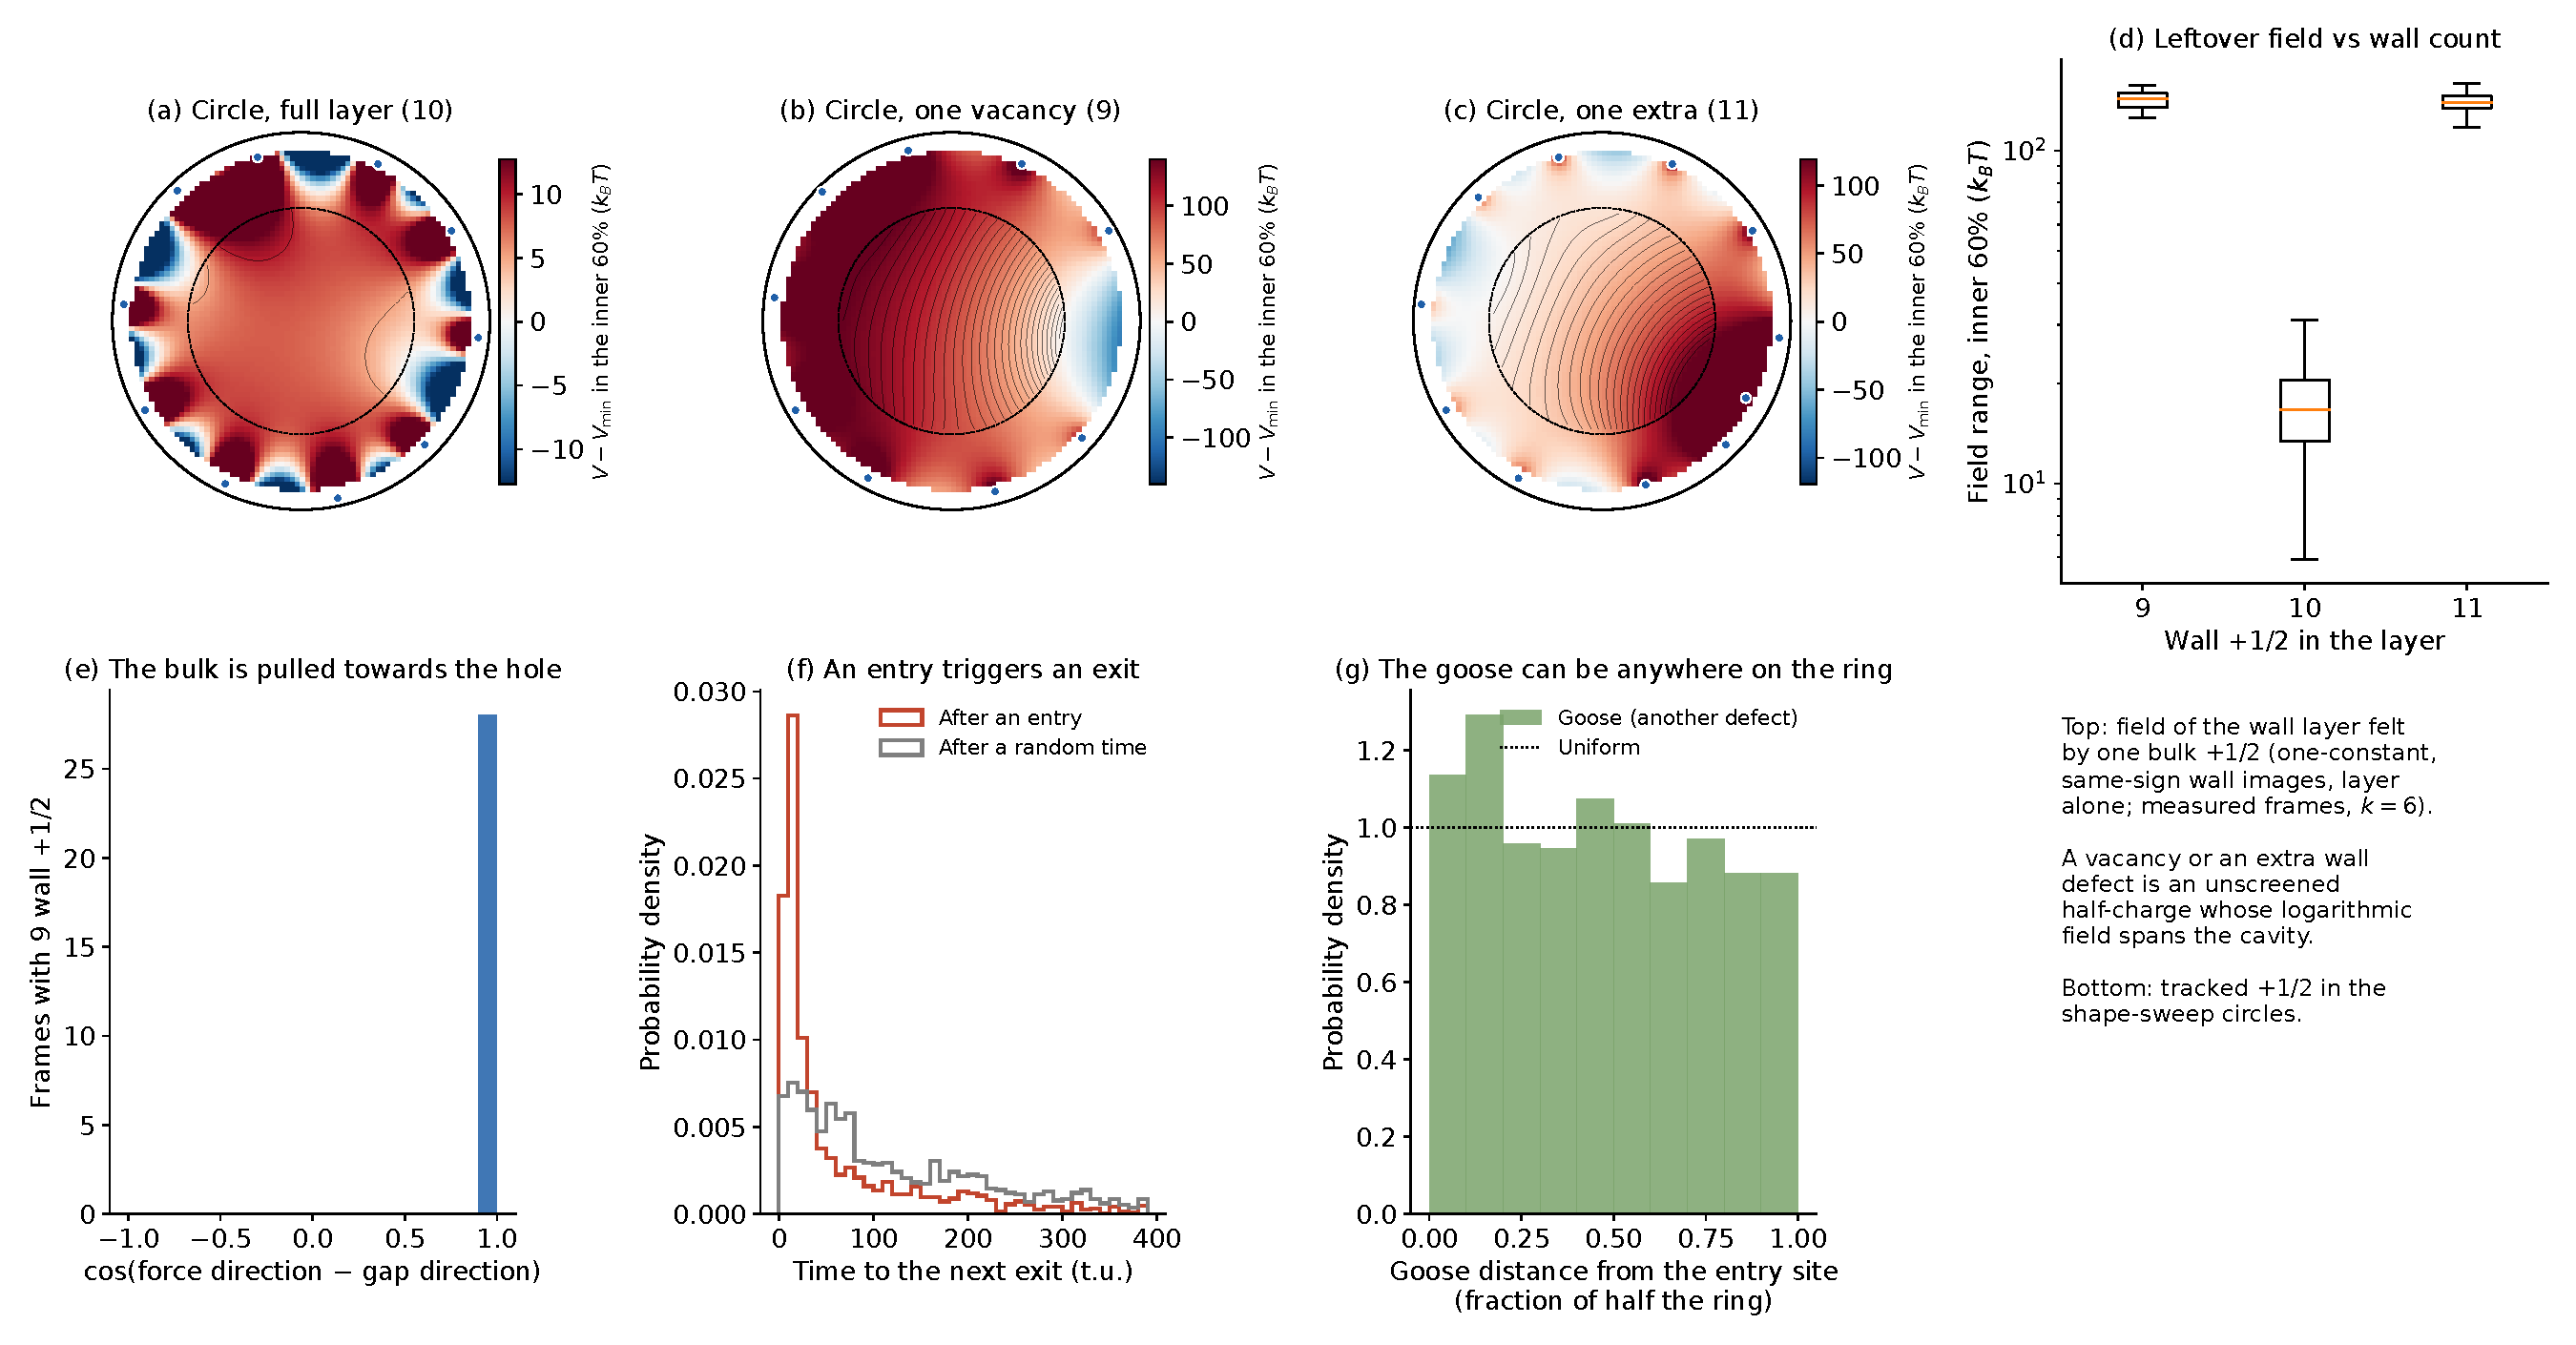
\includegraphics[width=\columnwidth]{fig_vacancy_field}
\caption{\todo{merge into Fig.~4 or SM}. Vacancy versus full layer in active circles. (a--e) $k=6$, area 2500; (f, g) shape-sweep circles, $R_{\rm eq}=1$--$1.5\,\la$, all $k$. (a--c) Field of the layer felt by one bulk $+\half$ for a full layer, one
vacancy and one extra wall defect; (d) its range inside $r<0.6R$ against the wall count; (e) with a vacancy the force on a bulk $+\half$ points at the hole;
(f) time to the next exit after an entry into the layer vs after a random time; (g) position of the defect that leaves (`goose') relative to the entry site.}\label{fig:vac}
\end{figure}

The released charge obeys a wall law (Fig.~\ref{fig:shapes}). Above aspect $\approx1.5$ the bulk charge per unit wall length no longer depends on shape or size
and is set by the winding density $q=k/P$ alone, $Q_b\approx c(q)P$, with $c\approx0.012$ at $q\approx0.03$; denser windings release a smaller fraction
(0.61 at $q=0.02$, 0.10 at $q=0.07$). A periodic channel with the same winding density, the flat limit of the cavities, releases the same share for widths $W\gtrsim18$ cells. Circles are the
exception: they hold exactly $+1$ up to $R\approx2\,\la$, the topologically protected case.

\paragraph*{Mirror control.} Reversing the winding ($k\to-k$) fills the wall layer with $-\half$ defects, which are not self-propelled. In the same 675 cavities the
coherent vortex breaks just as before (circulation $0.66\to0.1$ at $R_\mathrm{eq}=2\,\la$), but the $-\half$ layer does not leak: at aspect $\geq1.4$ it loses
$0.05$ defects relative to the circle (the $+\half$ layer loses 2, up to 4.7), and its escape rate is $\approx30\times$ lower [Fig.~\ref{fig:shapes}(g); SM Sec.~S13].
Losing the vortex is therefore not enough; the leak needs the wall defects' own jets. (In the circle the $-\half$ layer gains about 1.5 of the 2 defects predicted
by the continuum at $k=-6$, 13.5 of 14 at $R\approx1.25\,\la$, and the full 2 in crowded walls of larger circles; open.)

% --------------------------------------------------------------------------------------------
\paragraph*{Discussion.} Topology fixes how much charge an active nematic cavity holds; geometry decides where it goes. The count of wall defects is the largest ring that can
tilt as a whole, $2|k-1|$ for either sign of the winding, set by how the anchoring turns relative to the wall. The active flow is what makes this geometric constraint
bite: a coherent vortex imposes a common tilt, and the layer must reach the commensurate ring. The two effects are inseparable. Without coherent flow the geometry is
silent (passive cavities keep $2k$), and without the geometry the flow has nothing to select (the tilt would carry no cost). Flow alignment fixes the angle of the tilt,
but not the outcome, as elongated cavities show: there the vortex breaks, and stronger alignment (up to $\lambda=6$) does not restore the layer. Activity enters twice, by driving the
coherent flow and by the jets of the wall defects that empty the layer once the flow is lost. The same physics should apply to any flow-aligning active nematic in a
cavity with patterned anchoring: microtubule--kinesin nematics or cell monolayers in wells whose walls impose a winding should hold $2k-2$ tilted wall defects in disks
and leak in elongated wells, while a negative winding should not leak. Two questions remain open: what pins crowded layers below the flow-aligned tilt, and why sparse
$-\half$ layers retain their extra defects so poorly.
\todo{Benjamin: experimental references (patterned anchoring in wells; active nematics in confinement) and whether to name specific systems}

\begin{acknowledgments}
\todo{acknowledgments, funding, computing}
\end{acknowledgments}

\bibliography{../refs}

\end{document}
